\documentclass{revtex4-2}
\usepackage[colorlinks=true, urlcolor=blue]{hyperref}
\usepackage{amsmath}
\usepackage{graphicx}

\begin{document}
\title{Assignment 2: Physics of Compact Objects}
\author{Md Arif Shaikh}
\affiliation{International Centre for Theoretical Sciences, Bengaluru}
\email{arifshaikh.astro@gmail.com}
\date{\today}
\maketitle

\section*{Problem 1}
\label{sec:problem-1}
Derive the homology relations for the pressure $P$, temperature $T$ and luminosity $L$ (express them in terms of the mass $M$ and radius $R$, as well as the mean molecular weight $\mu$ of the gas particles). Compare these with the numerical results that you obtained in the previous section (Problem 4).\\

The central concept of the homology models is that they describe star swith internal structures that are in some way self-similar. Specifically, consider a pair of stars whose structures are described by unprimed and primed variables. In this pair of stars, we can identify homologous mass shells as having the same relative mass coordinate in each star:

\begin{equation}
  \label{eq:relative-mass-coordinate}
  \xi = m/M = m'/M'
\end{equation}
These stars are said to homologous if the relative radii of the homologous mass shells are also equal
\begin{equation}
  \label{eq:relative-radii}
  r(\xi)/R = r'(\xi)/R'(\xi)
\end{equation}
Now let's define the following variables
\begin{equation}
  \label{eq:mass-molecular-weight}
  x \equiv M/M', y \equiv \mu/\mu'.
\end{equation}
We also introduce following variables
\begin{equation}
  \label{eq:z-p-t-s}
  z = r(\xi)/r'(\xi) = R/R', p = P(\xi)/P'(\xi) = P_c/P_c', t = T(\xi)/T'(\xi)=T/T_c', s = l(\xi)/l'(\xi) = L/L'.
\end{equation}
The assumption here is that the ratios between the radii, pressures, temperatures and luminosities, for homologous mass shells, are constant and independent of $\xi$--these ratios depending only on which pair of stars are under consideration.

First let's remember the stellar structure equations
\begin{equation}
  \label{eq:hydrostatic}
  \begin{aligned}
    & \frac{dP}{dm_r} = \frac{-G m_r}{4\pi r^4} \\
    & \frac{dr}{dm_r} = \frac{1}{4\pi r^2 \rho}\\
    & \frac{dT}{dm_r} = \frac{-3k}{64\pi^2 ac} \frac{1}{T^3}\frac{L_r}{r^4}\\
    & \frac{dL_r}{dm_r} = \epsilon.
  \end{aligned}
\end{equation}
We want the $m_r$ to be written in terms of $m_r = m(r) = \xi M$, this would give
\begin{equation}
  \label{eq:hydrostatic-in-xi}
  \begin{aligned}
    & \frac{dP}{d\xi} = \frac{-G \xi M^2}{4\pi r^4} \\
    & \frac{dr}{d\xi} = \frac{M}{4\pi r^2 \rho}\\
    & \frac{dT}{d\xi} = \frac{-3k}{64\pi^2 ac} \frac{M}{T^3}\frac{L_r}{r^4}\\
    & \frac{dL_r}{d\xi} = \epsilon M.
  \end{aligned}
\end{equation}
Next we want to replace variables in terms of the primed variables using $z, p, t, s$ in \eqref{eq:z-p-t-s}. This would give
\begin{equation}
  \label{eq:hydrostatic-in-xi-primed}
  \begin{aligned}
    & \frac{dP'}{d\xi} = \frac{-G \xi M'^2}{4\pi r'^4}\left(\frac{x^2}{p z^4}\right)  \\
    & \frac{dr'}{d\xi} = \frac{M'}{4\pi r'^2 \rho'}\left(\frac{x}{z^3d}\right) \\
    & \frac{dT'}{d\xi} = \frac{-3k'}{64\pi^2 ac} \frac{M'}{T'^3}\frac{L_r'}{r'^4} \left(\frac{\kappa s x}{z^4 t^4}\right) \\
    & \frac{dL_r'}{d\xi} = \epsilon' M' \left(\frac{e x}{s}\right) .
  \end{aligned}
\end{equation}
where we have used
\begin{equation}
  e = \epsilon/\epsilon', \kappa = k/k', d = \rho/\rho'.
  \label{eq:e-kappa-d}
\end{equation}
In order that the primed variables obey the hydrostatic equilibrium equation, we need the quantity inside brackets to be equal to unity.
\begin{equation}
  \label{eq:homologous-condition}
  \frac{x^2}{pz^4} = 1, \frac{x}{z^3d} = 1, \frac{ksx}{z^4 t^4} = 1, \frac{ex}{s} = 1.
\end{equation}
First condition gives,
\begin{equation}
  \label{eq:pressure}
  \frac{P}{P'} = \frac{(M/M')^2}{(R/R')^4}.
\end{equation}
We need to get rid of the $k, e$ and $d$. For that, we first assume the following relations
\begin{equation}
  \label{eq:micro-physics}
  \rho\sim P^\alpha T^{-\delta}\mu^\varphi, \epsilon \sim \rho^\lambda T^\nu, \kappa \sim P^a T^b
\end{equation}
substituting this in the eq. \eqref{eq:e-kappa-d}, gives
\begin{equation}
  \label{eq:e-kappa-d-2}
  e = p^{\lambda\alpha} t^{\nu-\lambda\delta}y^{\lambda\varphi},\quad \kappa = p^a t^b,\quad d = p^\alpha t^{-\delta}y^\varphi. 
\end{equation}
We use these to substitute $e, \kappa$ and $d$ in eq. \eqref{eq:homologous-condition}. This will give
\begin{equation}
  \label{eq:homologous-condition-2}
  \frac{x^2}{pz^4} = 1, \frac{x t^\delta}{z^3 p^\alpha y^\varphi} = 1, \frac{p^a sx}{z^4 t^{4-b}} = 1, \frac{p^{\lambda\alpha} t^{\nu-\lambda\delta}y^{\lambda\varphi} x}{s} = 1.
\end{equation}
Now we have four unknown variables $z, p, t, s$ and two known variables $x, y$. We take a trial solution of the form
\begin{equation}
  \label{eq:trial}
  z = x^{z_1}y^{z_2},\quad p = x^{p_1}y^{p_2},\quad t = x^{t_1}y^{t_2},\quad s = x^{s_1}y^{s_2}.
\end{equation}
We use this in eq. \eqref{eq:homologous-condition-2} to get
\begin{equation}
  \label{eq:eq-set-1}
  \begin{aligned}
    & x^{2 - p_1 - 4z_1}y^{- p_2 - 4z_2} = 1,\\
    & x^{1 + \delta t_1 - 3 z_1 - \alpha p_1}y^{-\varphi + \delta t_2 - 3 z_2 - \alpha p_2} = 1,\\
    & x^{ap_1 + s_1 + 1 - 4z_1 + (b-4)t_1}y^{ap_2 + s_2 - 4 z_2 + (b-4)t_2} = 1,\\
    & x^{\lambda\alpha p_1 + (\nu-\lambda\delta) t_1 + 1 - s_1}y^{\lambda\alpha p_2 + (\nu-\lambda\delta) t_2 - s_2 + \lambda\varphi} = 1.
\end{aligned}
\end{equation}
Equating the powers to zero, gives then the following two sets of four equations
\begin{equation}
  \label{eq:eq-set-2}
  \begin{aligned}
    & 2 - p_1 - 4z_1 = 0, 1 + \delta t_1 - 3 z_1 - \alpha p_1 = 0, ap_1 + s_1 + 1 - 4z_1 + (b-4)t_1 = 0, \lambda\alpha p_1 + (\nu-\lambda\delta) t_1 + 1 - s_1\\
    & - p_2 - 4z_2 = 0, -\varphi + \delta t_2 - 3 z_2 - \alpha p_2 = 0, ap_2 + s_2 - 4 z_2 + (b-4)t_2 = 0, \lambda\alpha p_2 + (\nu-\lambda\delta) t_2 - s_2 + \lambda\varphi.
  \end{aligned}
\end{equation}
We can rewrite these as the following
\begin{equation}
  \label{eq:matrix-1}
  \begin{bmatrix}
    -4 & -1 & 0 & 0\\
    -3 & -\alpha & \delta & 0\\
    -4 & a & (b-4) & 1\\
    0 & \lambda\alpha & (\nu-\lambda\delta) & -1
  \end{bmatrix}
  \begin{bmatrix}
    z_1 \\
    p_1 \\
    t_1\\
    s_1
  \end{bmatrix} =
  \begin{bmatrix}
    -2\\
    -1\\
    -1\\
    -1
  \end{bmatrix}
\end{equation}

and similarly

\begin{equation}
  \label{eq:matrix-2}
  \begin{bmatrix}
    -4 & -1 & 0 & 0\\
    -3 & -\alpha & \delta & 0\\
    -4 & a & (b-4) & 1\\
    0 & \lambda\alpha & (\nu-\lambda\delta) & -1
  \end{bmatrix}
  \begin{bmatrix}
    z_2 \\
    p_2 \\
    t_2\\
    s_2
  \end{bmatrix} =
  \begin{bmatrix}
    0\\
    \varphi\\
    0\\
    -\lambda\varphi
  \end{bmatrix}
\end{equation}
The general solution for these sets of equation could be obtained using, e.g., Mathematica. The solution have a simpler form for ideal gas ($\alpha = \delta = \varphi = 1$) and a constant opacity $(a=b=0)$. The solutions in this case are (See the Mathematica notebook)
\begin{equation}
  \label{eq:sol-1}
  z_1 = \frac{\lambda +\nu -2}{3 \lambda +\nu },\quad p_1 = \frac{2 (\lambda -\nu +4)}{3 \lambda +\nu },\quad t_1 = \frac{2 (\lambda +1)}{3 \lambda +\nu },\quad s_1 = 3.
\end{equation}
and
\begin{equation}
  \label{eq:sol-2}
  z_2 = \frac{\nu -4}{3 \lambda +\nu },\quad p_2 =  -\frac{4 (\nu -4)}{3 \lambda +\nu },\quad t_2 = \frac{3 \lambda +4}{3 \lambda +\nu },\quad s_2 = 4.
\end{equation}

This means we have from \eqref{eq:trial},

\begin{equation}
  \label{eq:temperature-luminosity}
  \boxed{T/T' = t = (M/M')^{\left(\frac{2(\lambda + 1)}{3\lambda + \nu} \right)}(\mu/\mu')^{\frac{3 \lambda +4}{3 \lambda +\nu }}}\quad \boxed{L/L' = s = (M/M')^3 (\mu/\mu')^4}.
\end{equation}

\section*{Problem 2}
\label{sec:problem-2}
Form eq. \eqref{eq:pressure} we get $P \propto M^2/R^4$. Now $\rho \propto M/R^3$. Substituting $R$ one gets
\begin{equation}
  \label{eq:pressure-density}
  P \propto M^2 / (M/\rho)^{4/3} = M^{2/3}\rho^{4/3}.
\end{equation}

\section*{Problem 3}
\label{sec:problem-3}
Consider a slowly contracting star in quasi-hydrostatic equilibrium for which the pressure is given by a combination of ideal gas and electron degeneracy : $P = (\mathcal{R}/\mu_e)\rho T + K(\rho/\mu_e )^\gamma$ , where $\gamma$ varies between $5/3$ (non-relativistic) and $4/3$ (extreme relativistic). Plot the variation of $T_c$ with $\rho_c$.\\

From the previous problem we have $P_c = CG M^{2/3}\rho_c^{4/3}$. Using this we replace $P_c$ in pressure equation in the question to get an equation consisting of $\rho_c$ and $T_c$ only. This gives
\begin{equation}
  \label{eq:rho-T}
  CG M^{2/3}\rho_c^{4/3} = (\mathcal{R}/\mu_e)\rho_c T_c + K(\rho_c/\mu_e )^\gamma
\end{equation}
So $T_c$ could be easily written in terms of $\rho_c$ as
\begin{equation}
  \label{eq:Tc}
  T_c = \frac{\mu_e}{\mathcal{R}} \left(CGM^{2/3}\rho_c^{1/3} - K \rho_c^{\gamma-1}/\mu_e^\gamma\right).
\end{equation}
The value of $K$ changes smoothly with $\gamma$. $K_{\gamma = 4/3} = 1.24 \times 10^{15}$ and $K_{\gamma = 5/3} = 10^{13}$ in cgs units.
\begin{center}
  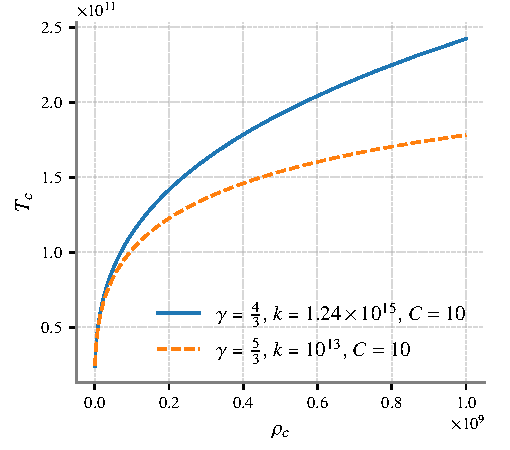
\includegraphics{./Tc_vs_rhoc.pdf}
\end{center}

\section*{Problem 4}
\label{sec:problem-4}
Derive an expression for the maximum central temperature reached by a star of mass $M$.

In the previous problem we derived the expression for $T_c$ in terms of $\rho_c$ and the other variables. To get the maximum $T_c$ we take the first derivative of it with respect to $\rho_c$ keeping other variables fixed. This is given by
\begin{equation}
  \label{eq:Tc-1}
  \frac{\partial T_c}{\partial \rho_c} = \frac{\mu _e}{\mathcal{R}} \left(\frac{C G M^{2/3}}{3 \rho _c^{2/3}}-(\gamma -1)
   K \rho _c^{\gamma -2} \mu _e^{-\gamma }\right)
\end{equation}
$T_c$ is maximum for
\begin{equation}
  \label{eq:rhoc-max}
  \rho_c^{\text{max}} = 27^{\frac{1}{4-3 \gamma }} \left(\frac{(\gamma -1) K \mu _e^{-\gamma
   }}{C G M^{2/3}}\right){}^{\frac{3}{4-3 \gamma }}
\end{equation}

Using this value in eq. \eqref{eq:Tc}, we get $T_c^{\text{max}}$
\begin{equation}
  \label{eq:Tc-max}
  T_c^{\text{max}} = \frac{\mu _e}{R} \left(C G M^{2/3} \sqrt[3]{27^{\frac{1}{4-3 \gamma }}
   \left(\frac{(\gamma -1) K \mu _e^{-\gamma }}{C G
   M^{2/3}}\right){}^{\frac{3}{4-3 \gamma }}}-K \mu _e^{-\gamma }
   \left(27^{\frac{1}{4-3 \gamma }} \left(\frac{(\gamma -1) K \mu _e^{-\gamma }}{C
   G M^{2/3}}\right){}^{\frac{3}{4-3 \gamma }}\right){}^{\gamma -1}\right)
\end{equation}


\end{document}